%\documentclass[draft]{beamer}
\documentclass{beamer}
  
\usepackage{thumbpdf}           % Thumbnails for PDF versions
\usepackage{hyperref}
\usepackage{pgf}
\usepackage{tikz}
\usepackage{bm}
\usepackage{movie15}
\usepackage{textcomp}

\definecolor{green::dark}{rgb}{0.,0.7,0}

\title{Advanced Amateur Radio Licence}
\author{Rupert Brooks}

%%%%%%%%%%%%%%%%%%%%%%%%%%%%%%%%%%%%%%%%%%%%%%%%%%%%%%%%%%%%%%%%%%%%%%%%%%%%%%%%%%
%\setbeamertemplate{navigation symbols}{}
%\setbeamertemplate{frametitle}[default][right]
\setbeamertemplate{frametitle}{
\begin{flushright}
\insertframetitle\\
{\small \insertframesubtitle}
\end{flushright}
}

\setbeamertemplate{footline}[frame number]

\usefonttheme{professionalfonts}

%\setbeamertemplate{background}
%{
%\put(-10,0){
%\includegraphics[height=0.2\paperwidth]{logo.jpg}
%}%
%\put(0,2){
%\includegraphics[width=0.5in]{MICCAI_Logo_CMYK.pdf}
%}


%%%%%%%%%%%%%%%%%%%%%%%%%%%%%%%%%%%%%%%%%%%%%%%%%%%%%%%%%%%%%%%%%%%%%%%%%%%%%%%%%%
\def\lemma{{\large  \usebeamercolor[fg]{titlelike} Lemma\\}}
\def\proof{{\large  \usebeamercolor[fg]{titlelike}  Proof\\}}
\def\endproof{\qed}

\def\point#1{{\large  \usebeamercolor[fg]{titlelike}  #1\\}}
\def\herepoint#1{{\large  \usebeamercolor[fg]{titlelike}  #1}}

\def\emph#1{{\usebeamercolor[fg]{titlelike}  #1}}

%%%%%%%%%%%%%%%%%%%%%%%%%%%%%%%%%%%%%%%%%%%%%%%%%%%%%%%%%%%%%%%%%%%%%%%%%%%%%%%%%%
\begin{document}

%%%%%%%%%%%%%%%%%%%%%%%%%%%%%%%%%%%%%%%%%%%%%%%%%%%%%%%%%%%%%%%%%%%%%%%%%%%%%%%%%%
\begin{frame}
\maketitle
\end{frame}


%%%%%%%%%%%%%%%%%%%%%%%%%%%%%%%%%%%%%%%%%%%%%%%%%%%%%%%%%%%%%%%%%%%%%%%%%%%%%%%%%%
%% \section*{Outline}
%% \begin{frame}[allowframebreaks]
%% \frametitle{Outline}
%% \tableofcontents
%% \end{frame}
%%%%%%%%%%%%%%%%%%%%%%%%%%%%%%%%%%%%%%%%%%%%%%%%%%%%%%%%%%%%%%%%%%%%%%%%%%%%%%%%%%

\section*{Outline}

\begin{frame}{Outline}{}
\tableofcontents
\end{frame}
%%%%%%%%%%%%%%%%%%%%%%%%%%%%%%%%%%%%%%%%%%%%%%%%%%%%%%%%%%%%%%%%%%%%%%%%%%%%%%%%%%
\section{Prolegomena}

\subsection{Basics}
\begin{frame}{Units}{}
\begin{itemize}
\item Farad: Capacitance,$1F=1C/V=1s^4 \cdot A^2/m^2 \cdot kg$  
\item Henry: Inductance, $1H=1Wb/A=1V \cdot s/A=1\Omega\cdot s$
\item Hertz: Frequency, $f$, also angular frequency $\omega$ in $rad/s$
\item $1Hz=2\pi rad/s; f=2\pi\omega$
\end{itemize}
\end{frame}

\begin{frame}{Concepts}{}
\begin{itemize}
\item Skin Effect: RF current in a conductor flows along the outside
\end{itemize}
\end{frame}
%%%%%%%%%%%%%%%%%%%%%%%%%%%%%%%%%%%%%%%%%%%%%%%%%%%%%%%%%%%%%%%%%%%%%%%%%%%%%%%%%%

\section{RLC Circuits}

\subsection{Time Constant}
\begin{frame}{Time Constant}{}
\begin{itemize}
\item Time constant: 
\begin{itemize}
\item RC – time required for voltage to reach 63.2\% of equilibrium
\item RL – time required for current to reach 63.2\% of equilibrium
\end{itemize}
\item Why 63.2\%?  Because it is an exponential function.
\end{itemize}
\parbox{0.48\textwidth}{

\[v(t)=v_e e^{-t/RC}\]
}
\parbox{0.48\textwidth}{

\[I(t)=I_e e^{-tL/R}\]
}
Note: These are both for decay.  For rise, use $1-e^{-t/RC}$
\end{frame}

\begin{frame}{Time Constant}{}
\begin{tabular}{ccc}
Time constants & $e^{-t}$ & $1-e^{-t}$ \\
\hline  
0&	1.000&	0.000\\
1&	0.368&	0.632\\
2&	0.135&	0.865\\
3&	0.050&	0.950\\
4&	0.018&	0.982\\
5&	0.007&	0.993\\
\hline
\end{tabular}

\begin{itemize}
\item Circuitlab RC \url{https://www.circuitlab.com/circuit/ga5y34/simple-rc/}
\item Circuitlab RL \url{https://www.circuitlab.com/circuit/veg4ma/simple-rl/}
\end{itemize}
\end{frame}

\subsection{Reactance}
\begin{frame}{Reactance}{}
\begin{itemize}
\item In a pure resistance, current is in phase with voltage.
\item In a pure capacitance, current leads voltage by 90\textdegree
\item In a pure inductance, voltage leads current by 90\textdegree
\item Reactance and resistance can be viewed as a complex number. Impedance is the magnitude of this number.
\end{itemize}

\parbox{0.48\textwidth}{

Capacitive Reactance

$X_c=\frac{-j}{2\pi fC}$
}
\parbox{0.48\textwidth}{
Inductive Reactance

$X_i=j2\pi fL$
}
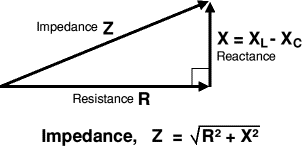
\includegraphics[width=0.4\textwidth]{images/imped.png}

Image taken from \url{http://electronicsclub.info/impedance.htm}
\end{frame}

\begin{frame}{Resonance}{}
\begin{itemize}
\item Capacitive and Inductive reactances oppose.
\item The frequency at which they exactly cancel is the resonant frequency.
\item $f=\frac{1}{2\pi\sqrt{LC}}$
\item The resonant frequency can be altered by resistance in some configurations, but not in pure series or pure parallel. 
\end{itemize}

\parbox{0.48\textwidth}{
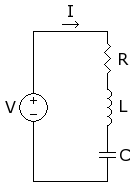
\includegraphics[width=0.2\textwidth]{images/RLC_series_circuit.png}
Attrib: \url{http://en.wikipedia.org/wiki/File:RLC_series_circuit.png}
}
\parbox{0.48\textwidth}{
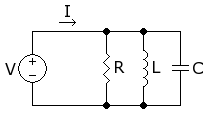
\includegraphics[width=0.4\textwidth]{images/RLC_parallel_circuit.png}
Attrib: \url{http://en.wikipedia.org/wiki/File:RLC_parallel_circuit.png}
}
\end{frame}
\begin{frame}{Q factor}{}
\begin{itemize}
\item Indication of 'quality' of a resonator.
\item High Q indicates small bandwidth, and low damping.
\item $Q=\frac{1}{F_b}$
\item Series $Q=\frac{X}{R}$, Parallel $Q=\frac{R}{X}$
\item $F_b$ is width between the -3dB points
\end{itemize}

\end{frame}

\begin{frame}{Examples on circuitlab}{}
\begin{itemize}
\item \url{https://www.circuitlab.com/circuit/5xp69v/series-rlc/}
\item \url{https://www.circuitlab.com/circuit/tgbk77/parallel-rlc/}
\end{itemize}
\end{frame}
%%%%%%%%%%%%%%%%%%%%%%%%%%%%%%%%%%%%%%%%%%%%%%%%%%%%%%%%%%%%%%%%%%%%%%%%%%%%%%%%%%

\section{Power Supplies}

\subsection{Rectifiers}
\begin{frame}{Rectifiers}{}
\begin{itemize}
\item Half Wave
\item Full Wave
\item Bridge
\end{itemize}
Note that the full wave is two diodes, one from each side of a center tapped transformer.  Thus the full wave has 
half the output voltage of a bridge (4 diodes).

Also, dont be tricked by the ripple frequency - its double the supply frequency for full and bridge rectifiers.

Diodes should be rated with a PIV of 2.8 times the transformer secondary.  Just memorize it.

They state you may put bypass resistors and capacitors around the rectifiers to guard against voltage spikes.  I have not seen this.
\end{frame}

\subsection{Filters}
\begin{frame}{Filters}{}
Supply filters are classified by the first component after the rectifer. 
\begin{itemize}
\item Choke input
\item Capacitor input 
\end{itemize}

Capacitor input has higher output voltage, but choke input can handle higher loads.

The questions state that choke input can give better regulation.

\end{frame}

\subsection{Terms and concepts}
\begin{frame}{Terms and concepts}{}
\begin{itemize}
\item {\em Bleeder Resistors} - maintain a minimum current draw, often necessary on choke input filtered systems
\item {\em Linear} vs {\em Switching} supplies
\item {\em Zener diodes} - often used as voltage reference
\item {\em Remote sensing.}  It may be necessary to take feedback from near the load, if the voltage may be drawn down over long supply leads.
\item {\em dynamic regulation} Managing short term changes in load resistance.
\item {\em static regulation} Managing long term changes in load resistance.
\end{itemize}

\end{frame}

\begin{frame}{Linear regulators}{}
\begin{itemize}
\item May be configured as series (series with load) or shunt (parallel with load) configuration.
\item Often packaged as a {\em three terminal regulator}.  
\item Internally, this contains
\begin{itemize}
\item voltage reference
\item error amplifier
\item sensing resistors and transistors
\item pass element
\end{itemize} 
\item and is characterized by
\begin{itemize}
\item min / max input voltage
\item max output current and max output voltage.
\end{itemize} 
\end{itemize}

\end{frame}


%%%%%%%%%%%%%%%%%%%%%%%%%%%%%%%%%%%%%%%%%%%%%%%%%%%%%%%%%%%%%%%%%%%%%%%%%%%%%%%%%%
\end{document}
 
